%%%%%%%%%%%%%%%%%%%%%%%%%%%%%%%%%%%%%%%%%
% Beamer Presentation
% LaTeX Template
% Version 1.0 (10/11/12)
%
% This template has been downloaded from:
% http://www.LaTeXTemplates.com
%
% License:
% CC BY-NC-SA 3.0 (http://creativecommons.org/licenses/by-nc-sa/3.0/)
%
%%%%%%%%%%%%%%%%%%%%%%%%%%%%%%%%%%%%%%%%%

%----------------------------------------------------------------------------------------
%	PACKAGES AND THEMES
%----------------------------------------------------------------------------------------

\documentclass[compress]{beamer}

\mode<presentation> {
\setbeamertemplate{headline}{}
% The Beamer class comes with a number of default slide themes
% which change the colors and layouts of slides. Below this is a list
% of all the themes, uncomment each in turn to see what they look like.

%\usetheme{default}
% \usetheme{AnnArbor}
%\usetheme{Antibes}
%\usetheme{Bergen}
%\usetheme{Berkeley}
%\usetheme{Berlin}
%\usetheme{Boadilla}
%\usetheme{CambridgeUS}
%\usetheme{Copenhagen}
%\usetheme{Darmstadt}
%\usetheme{Dresden}
%\usetheme{Frankfurt}
%\usetheme{Goettingen}
%\usetheme{Hannover}
%\usetheme{Ilmenau}
%\usetheme{JuanLesPins}
%\usetheme{Luebeck}
%\usetheme{Madrid}
%\usetheme{Malmoe}
%\usetheme{Marburg}
%\usetheme{Montpellier}
%\usetheme{PaloAlto}
%\usetheme{Pittsburgh}
%\usetheme{Rochester}
%\usetheme{Singapore}
%\usetheme{Szeged}
\usetheme{Warsaw}

% As well as themes, the Beamer class has a number of color themes
% for any slide theme. Uncomment each of these in turn to see how it
% changes the colors of your current slide theme.

%\usecolortheme{albatross}
%\usecolortheme{beaver}
%\usecolortheme{beetle}
%\usecolortheme{crane}
%\usecolortheme{dolphin}
%\usecolortheme{dove}
%\usecolortheme{fly}
%\usecolortheme{lily}
%\usecolortheme{orchid}
%\usecolortheme{rose}
\usecolortheme{seagull}
%\usecolortheme{seahorse}
%\usecolortheme{whale}
%\usecolortheme{wolverine}

%\setbeamertemplate{footline} % To remove the footer line in all slides uncomment this line
%\setbeamertemplate{footline}[page number] % To replace the footer line in all slides with a simple slide count uncomment this line

%\setbeamertemplate{navigation symbols}{} % To remove the navigation symbols from the bottom of all slides uncomment this line
}

\usepackage{graphicx} % Allows including images
\usepackage{booktabs} % Allows the use of \toprule, \midrule andxs                      % \bottomrule in tables
\usepackage{float}
\usepackage{caption}
\usepackage{subcaption}
\usepackage{listings} %syntax highlighting?
\usepackage{minted}
\usepackage{multicol} % table of contents
%\usepackage{subfigure}

%----------------------------------------------------------------------------------------
\graphicspath{ {./images/} }%	TITLE PAGE
%----------------------------------------------------------------------------------------
% \definecolor{mygreen}{cmyk}{0.82,0.11,1,0.25}
% \setbeamertemplate{blocks}[rounded][shadow=false]
% \addtobeamertemplate{block begin}{\pgfsetfillopacity{0.8}}{\pgfsetfillopacity{1}}
% \setbeamercolor{structure}{fg=mygreen}
\setbeamercolor*{block title example}{fg=black,
bg= gray!30}
\setbeamercolor*{block body example}{fg= black,
bg= gray!15}
\graphicspath{ {./images/}{./}{./timgs/} }

\title[RobotWords]{Learning how to talk robot.} % The short title appears at the bottom of every slide, the full title is only on the title page

\author{Katherine Scott} % Your name

\institute[Computer Vision Engineer] % Your institution as it will appear on the bottom of every slide, may be shorthand to save space
{
Computer Vision Engineer
\medskip
\textit{katherine.a.scott@gmail.com}
\textit{http://www.kscottz.com}
}
\date{\today} % Date, can be changed to a custom date

\begin{document}

\begin{frame}
\titlepage % Print the title page as the first slide
\end{frame}

% \begin{frame}
%   \frametitle{Outline}
%   %\tableofcontents[pausesections,subsectionstyle=hide]
%   \tableofcontents[currentsection,sectionstyle=show,subsectionstyle=hide]
%   % You might wish to add the option [pausesections]
% \end{frame}

% \begin{frame}%{\contentsname}
% %\begin{multicols}{2}
% \frametitle{Overview} % Table of contents slide, comment this block out to remove it
% \tableofcontents % Throughout your presentation, if you choose to use \section{} and \subsection{} commands, these will automatically be printed on this slide as an overview of your presentation
% %\end{multicols}
% \end{frame}

%----------------------------------------------------------------------------------------
%	PRESENTATION SLIDES
%----------------------------------------------------------------------------------------
\section{What is the most important language in robotics?}
\begin{frame}
  \frametitle{What is the most important language in robotics?}
  \begin{itemize}
  \item C++?
  \item Java?
  \item Python?
  \item Lisp?
  \item Assembly?
  \end{itemize}
\end{frame}
%----------------------------------------------------------------------------------------
\begin{frame}
   \frametitle{What is the most important language in robotics?}
   \begin{figure}
     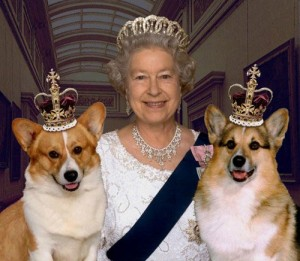
\includegraphics[width=0.5\linewidth]{corgis.jpg}
   \end{figure}
   \center{\huge{English!}}
 \end{frame}
%----------------------------------------------------------------------------------------
\begin{frame}
  \frametitle{So what is the most important skills of a roboticist?}
  \begin{figure}
     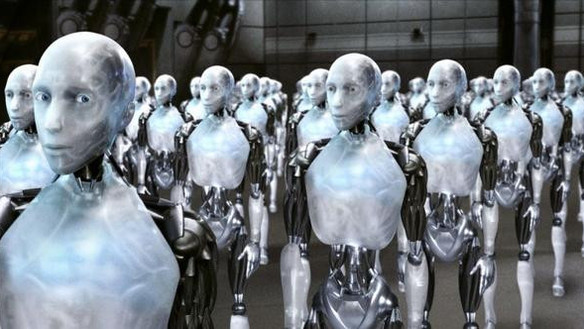
\includegraphics[width=0.5\linewidth]{robot-army.jpg}
   \end{figure}
   \begin{itemize}
   \item Mechanical Engineering?
   \item Electrical Engineering?
   \item Computer Science?
   \item Management?
   \item Protecting humans from the robot forthcoming robot apocalypse?
   \end{itemize}
 \end{frame}
%----------------------------------------------------------------------------------------
\begin{frame}
   \frametitle{So what is the most important skills of a roboticist?}
   \begin{figure}
     
\includegraphics[width=0.5\linewidth]{howdoishotweb.jpg}
   \end{figure}

   \begin{itemize}
     \item Asking the right question in the correct way.
     \item Finding and reading about a solution.
     \item Not being afraid to give it a shot.
   \end{itemize}
 \end{frame}
%----------------------------------------------------------------------------------------
\begin{frame}
   \frametitle{What I've learned.}
   \begin{figure}
     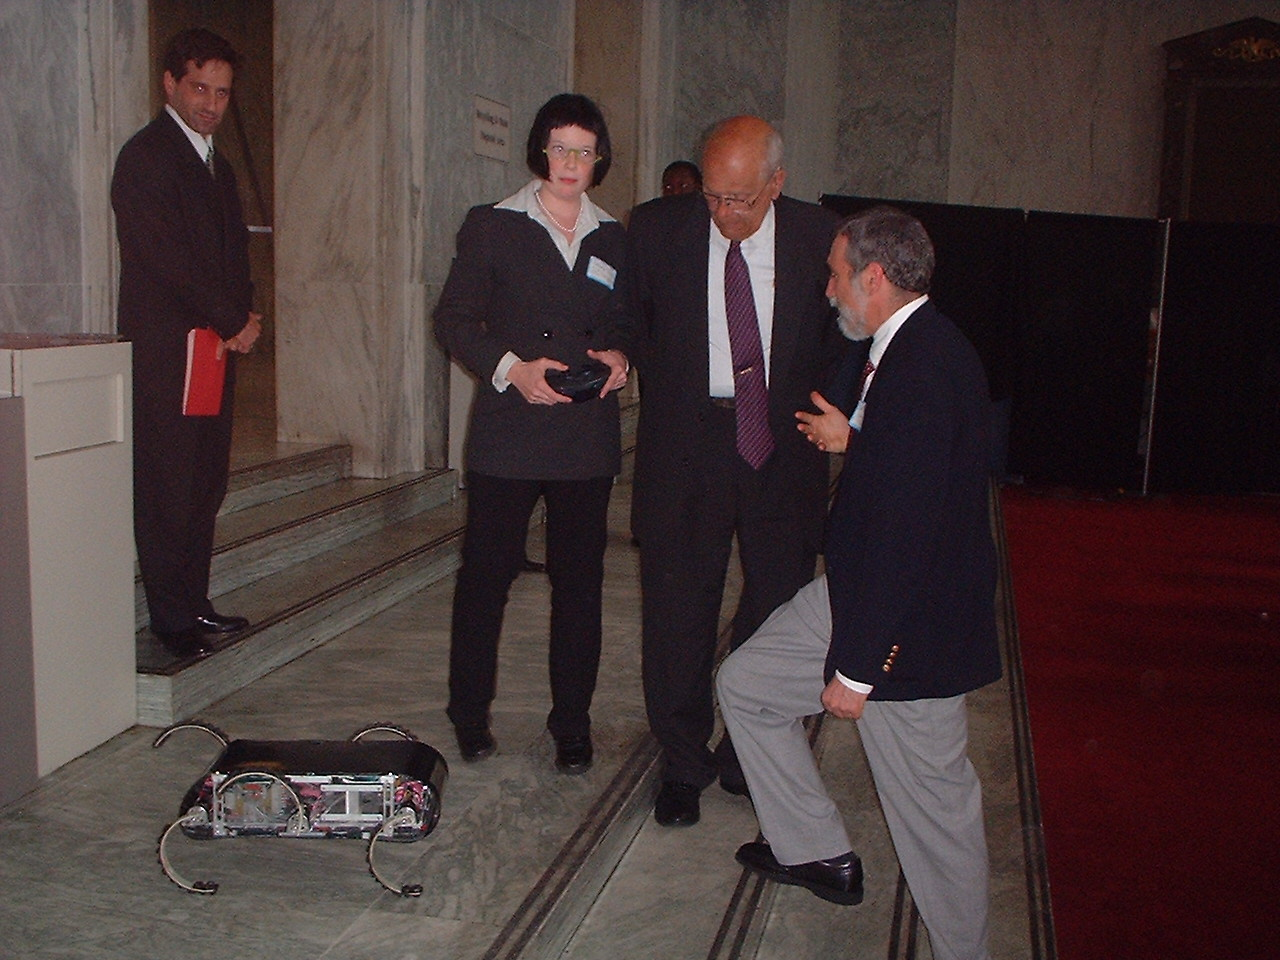
\includegraphics[width=0.5\linewidth]{youngkat.jpg}
   \end{figure}

   \begin{itemize}
     \item Words have \textbf{specific} meaning. Learn the meaning.
     \item With these words you can ask (google) better questions. 
     \item These words encode scientific papers that you can read.
     \item You start to sound like a pro. People will respect your opinion.
   \end{itemize}
 \end{frame}
%----------------------------------------------------------------------------------------
\begin{frame}
   \frametitle{What I've learned... about math}
   \begin{figure}
     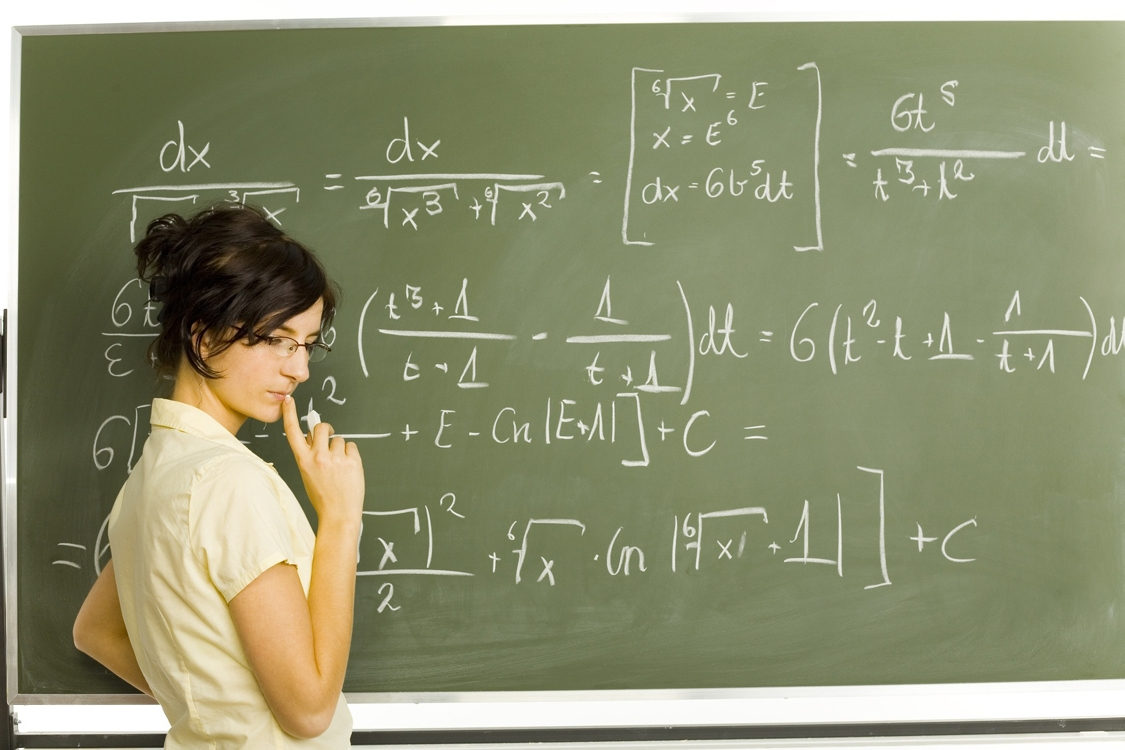
\includegraphics[width=0.5\linewidth]{math.jpg}
   \end{figure}

   \begin{itemize}
   \item \textbf{Learn to skim scientific papers}. 
     \item Math is just another language. Learn the symbols to unlock the meaning.
     
     \item Remember, you don't have to do the math (proof, derivation, etc), you just need to translate it to code or English. 
   \end{itemize}
 \end{frame}
%----------------------------------------------------------------------------------------
\begin{frame}
   \frametitle{And another thing!}
   \begin{figure}
     
\includegraphics[width=0.3\linewidth]{DontPanic.jpg}
     \quad 
     
\includegraphics[width=0.3\linewidth]{rtfm.jpg}
   \end{figure}

   \begin{itemize}
   \item \textbf{DO NOT PANIC}
   \item \textbf{RTFM} READ THE FRAKING MANUAL. Really read it. Twice. 
   \item Break problems/solutions/papers down to the individual words, and work back up. 
   \item Ask for help.

   \end{itemize}
 \end{frame}
%----------------------------------------------------------------------------------------
\section{So let's learn some robot words to get you started.}
%----------------------------------------------------------------------------------------
\begin{frame}
   \frametitle{I brought my friend tapsterbot to help us.}
   \begin{figure}
     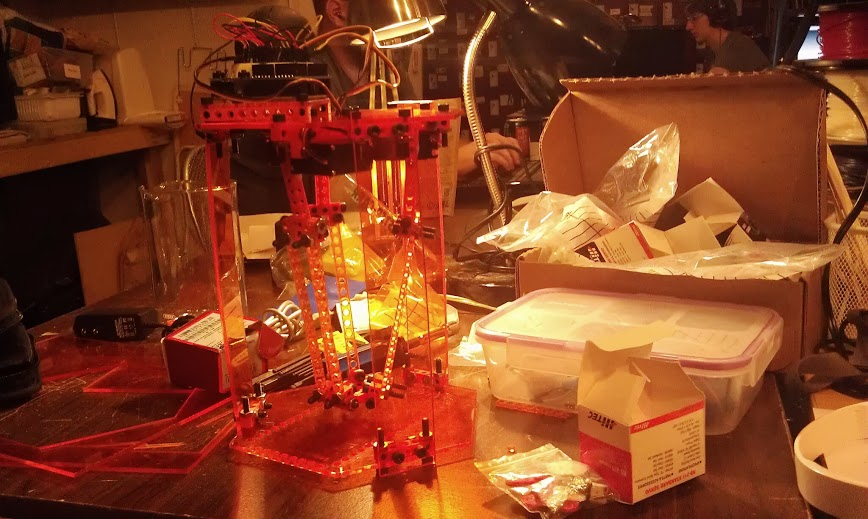
\includegraphics[width=0.7\linewidth]{tapster.jpg}
   \end{figure}

   \begin{itemize}
   \item Tapsterbot is a free and open-source parallel robot. 
   \item These types of robots are used for sorting tasks.
   \item Tapsterbot is used to automatically test smart phones.
   \item Cheap and easy to build. Just an arduino and a few servos.
   \end{itemize}
 \end{frame}
%----------------------------------------------------------------------------------------
\begin{frame}
   \frametitle{All Robots Have Three Basic Parts}
   \begin{itemize}
   \item \textbf{Sensors}
     \begin{itemize}
       \item Sense the world around the robot.
       \item Just like your eyes, ears, nose, and skin.
     \end{itemize}
   \item \textbf{Actuators}
     \begin{itemize}
       \item Move the robot around. Motors, gears, levers, cams, etc.
       \item Just like your muscles and bones.
     \end{itemize}     
   \item \textbf{Controllers} 
     \begin{itemize}
       \item Take input from sensors, reason about it, and decide what to do.
       \item Just like your brain. 
     \end{itemize}          
   \end{itemize}     
 \end{frame}
%----------------------------------------------------------------------------------------
\begin{frame}
   \frametitle{Let's look at tapsterbot}
   \begin{figure}
     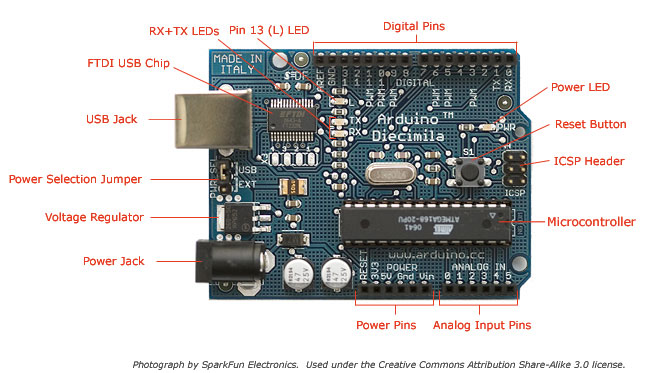
\includegraphics[width=0.45\linewidth]{arduino.jpg}
     \quad 
     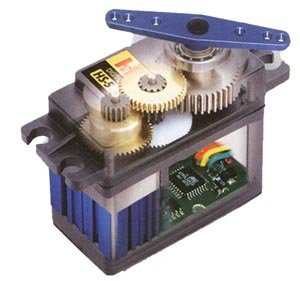
\includegraphics[width=0.25\linewidth]{hitec.jpg}
   \end{figure}

   \begin{itemize}
   \item \textbf{Sensors}
     \begin{itemize}
       \item Eventually a camera on top.
       \item Each servo has an encoder.
     \end{itemize}
   \item \textbf{Actuators}
     \begin{itemize}
       \item Hobby servos (servos have built in sensors).
     \end{itemize}     
   \item \textbf{Controllers} 
     \begin{itemize}
       \item Arduino connected to my computer.
     \end{itemize}          
   \end{itemize}     
 \end{frame}
%----------------------------------------------------------------------------------------
\begin{frame}
  \frametitle{Other things robots usually have...}
   \begin{figure}
     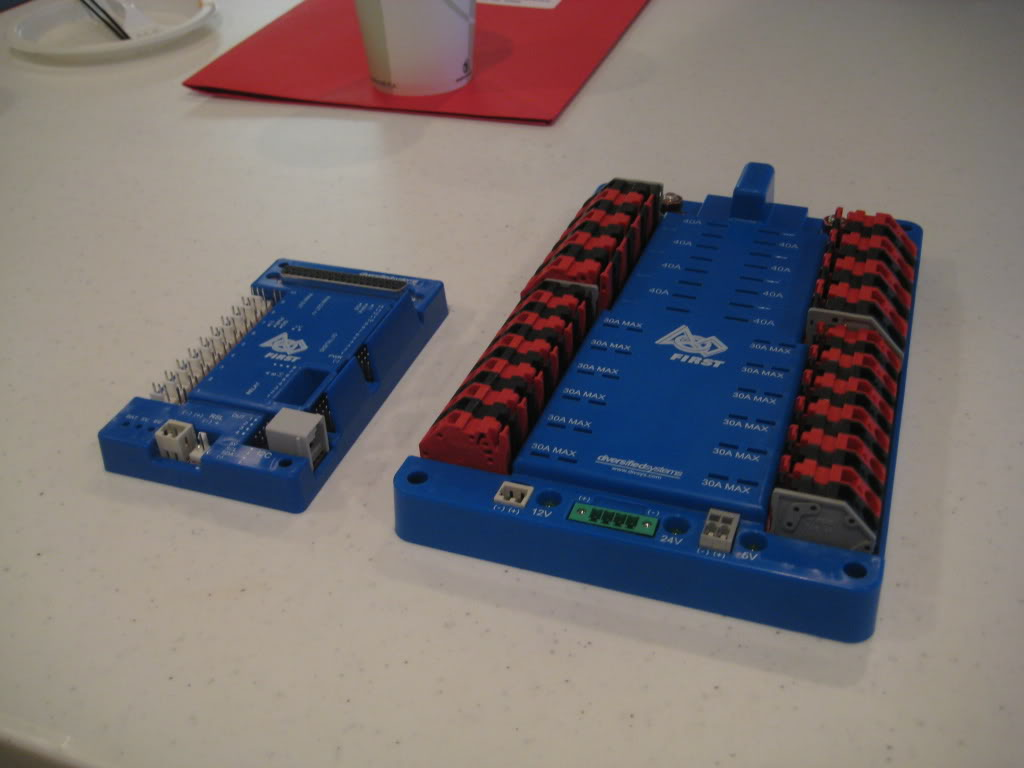
\includegraphics[width=0.4\linewidth]{frc.jpg}
   \end{figure}

   \begin{itemize}
   \item \textbf{Power Distribution}
     \begin{itemize}
       \item Different parts take different voltages, current but come from one battery.
     \end{itemize}
   \item \textbf{Digital IO}
     \begin{itemize}
       \item This board usually translates (talks) in different digital and analog formats.
     \end{itemize}     
   \item \textbf{Communications} 
     \begin{itemize}
       \item How do we control the robot remotely. Usually wifi.
     \end{itemize}
     \item On tapsterbot the Arduino does most of this stuff. 
   \end{itemize}     
 \end{frame}
%----------------------------------------------------------------------------------------
\begin{frame}
  \frametitle{Common Sensors}
    
   \begin{figure}
     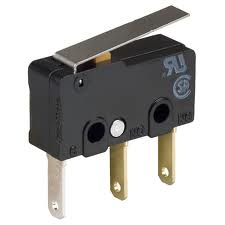
\includegraphics[width=0.2\linewidth]{limit.jpg}
     \quad
     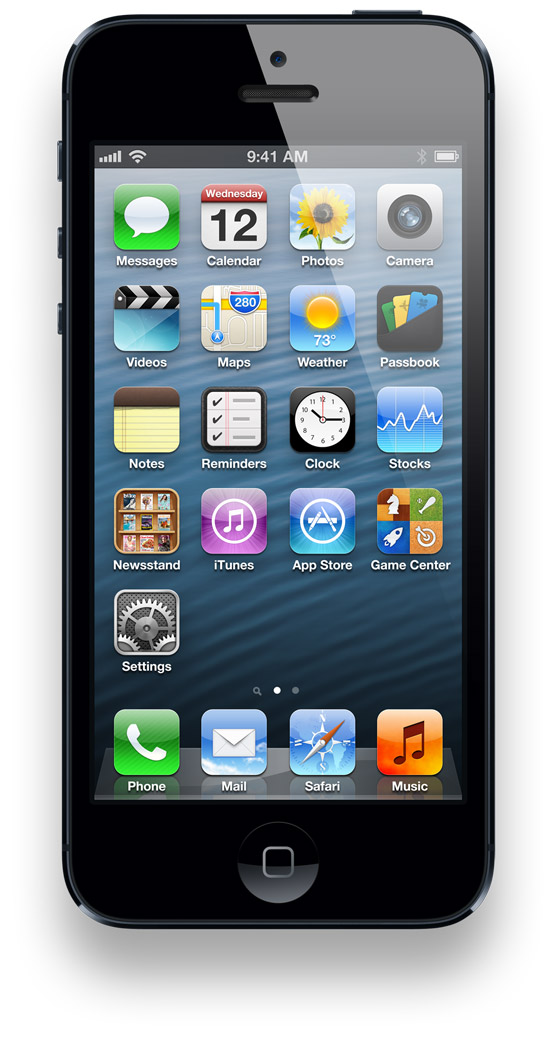
\includegraphics[width=0.1\linewidth]{iphone.jpg}
     \quad
     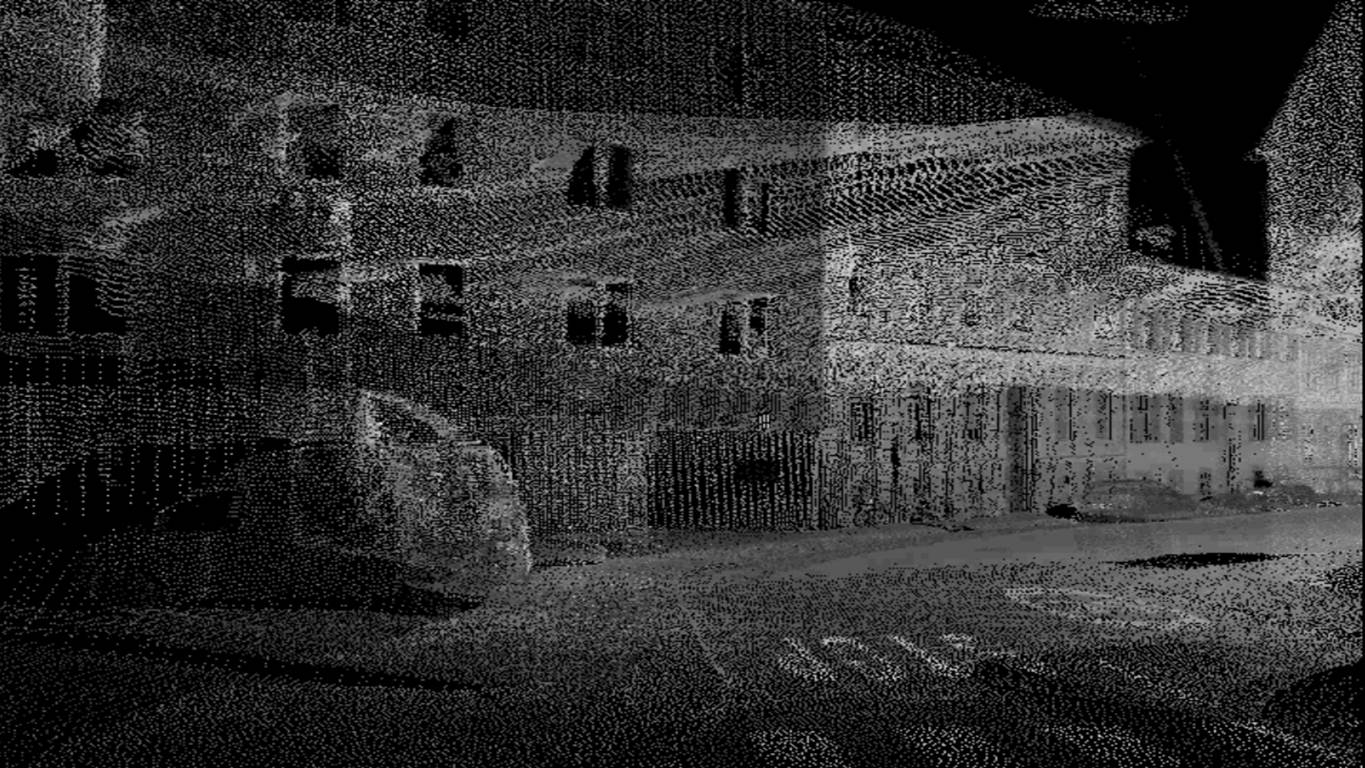
\includegraphics[width=0.3\linewidth]{lidar.jpg}
   \end{figure}
   \begin{itemize}
   \item \textbf{Encoders} - count how far something has moved (wheels).
   \item \textbf{Cameras} - see the world, stereo cameras give depth.
   \item \textbf{LIDAR} - Laser RADAR high fidelity 2D/3D maps.
   \item \textbf{Limit Switch} - Just a switch. Off or On.
   \item \textbf{Accelerometer} - Measures motion, can find gravity (down).
   \item \textbf{Gyroscope} - Measure rotation.
   \item \textbf{Magnetometers} - Can find North, metal stuff. 
   \end{itemize}     
 \end{frame}
%----------------------------------------------------------------------------------------
\begin{frame}
  \frametitle{Sensor Concepts}
  \begin{figure}
     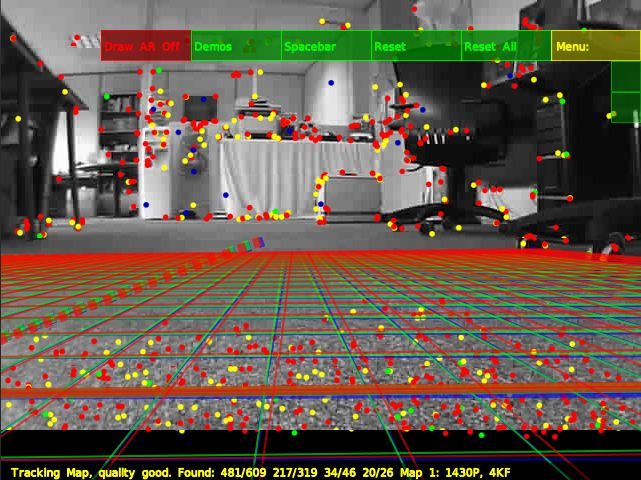
\includegraphics[width=0.4\linewidth]{ptam.jpg}
  \end{figure}

   \begin{itemize}
   \item \textbf{SLAM} - \href{http://www.youtube.com/watch?v=Y9HMn6bd-v8}{imultaneous localization and mapping.} Where am I?
   \item \textbf{Pose Tracking} - Figure out x,y,z location and orientation.
   \item \textbf{Sample Rate} - How fast? Measured in hertz (Hz). 
   \item \textbf{State} - What is the current pose of the robot.
   \item \textbf{Format} - What language does the sensor talk.
   \item \textbf{Calibration} - Does the sensor value match the real world. 
   \end{itemize}     
 \end{frame}
%----------------------------------------------------------------------------------------
\begin{frame}
  \frametitle{Types of Actuators}
  \begin{figure}
     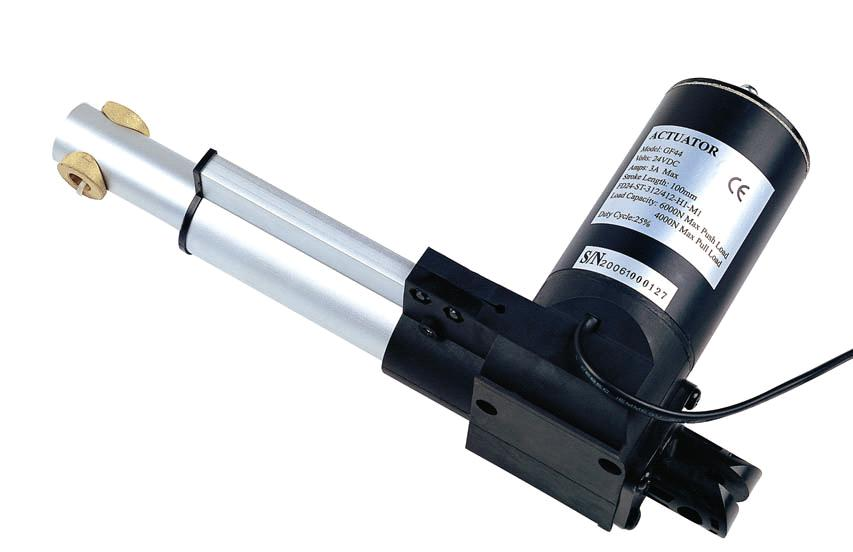
\includegraphics[width=0.2\linewidth]{linear.jpg}
     \quad
     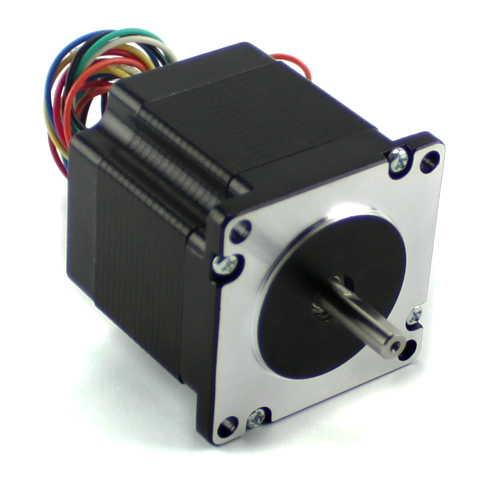
\includegraphics[width=0.2\linewidth]{stepper.jpg}
  \end{figure}
   \begin{itemize}
   \item \textbf{Things that look like motors} 
     \begin{itemize}
     \item \textbf{Motor} - A regular motor, might add an encoder.
     \item \textbf{Stepper} - A motor with an encoder that let's you do precise rotation.
     \item \textbf{Servo} - A motor with an encoder that turns a set number of degrees.
     \end{itemize}
   \item \textbf{Linear Actuator} - Motor that moves in a straight line. 
     \begin{itemize}
     \item \textbf{Pneumatics} - Linear actuators that move with air.
     \item \textbf{Hydraulics} - Linear actuators that move with oil or water.
     \end{itemize}     
   \end{itemize}     
 \end{frame}
%----------------------------------------------------------------------------------------
\begin{frame}
  \frametitle{Actuator Concepts}
  \begin{figure}
     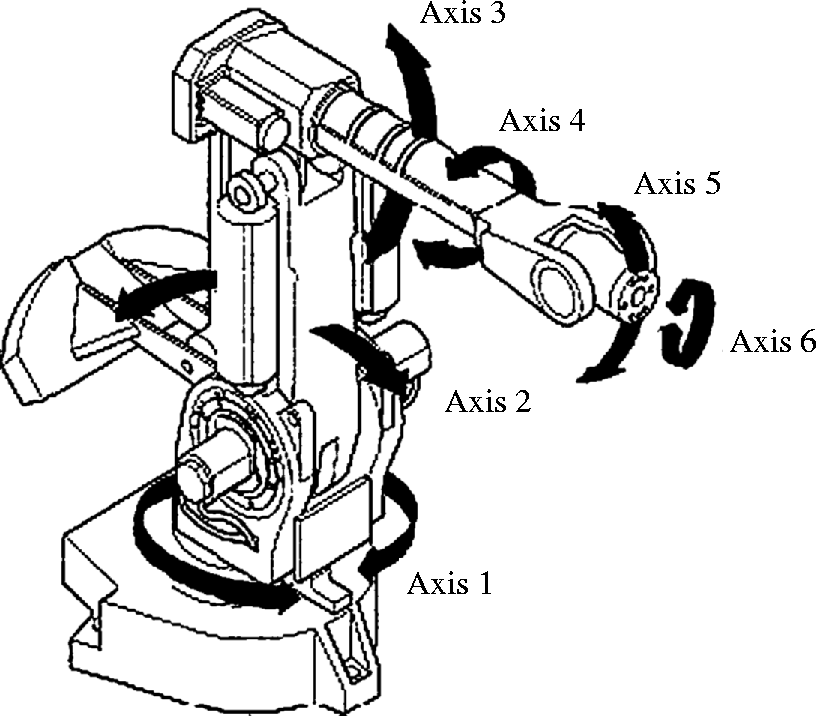
\includegraphics[width=0.4\linewidth]{6DOF.png}
     \quad
     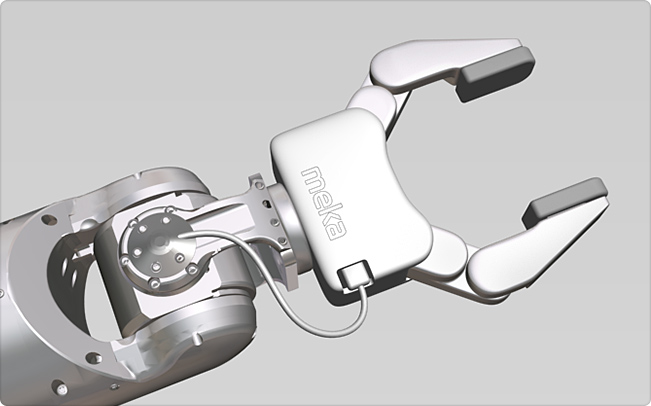
\includegraphics[width=0.4\linewidth]{gripper.jpg}
  \end{figure}
   \begin{itemize}
   \item Robots that move around are classified by how they move.
   \item \textbf{Degrees of Freedom - DOF} robots are also described by the number of things that move on them. 
   \item \textbf{End Effector} is a fancy word for a robotic hand. 
   \item How many degrees of freedom in tapsterbot?
   \end{itemize}     
 \end{frame}
%----------------------------------------------------------------------------------------
\begin{frame}
  \frametitle{Controllers - This is where the magic happens.}
  \begin{figure}
     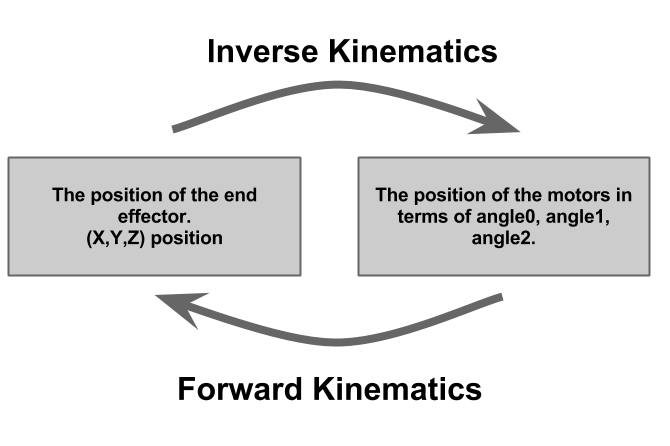
\includegraphics[width=0.4\linewidth]{kinematics.png}
  \end{figure}
   \begin{itemize}
   \item We use kinematic equations to relate points in the world to actuator positions. 
   \item \textbf{Forward Kinematics} - Forward kinematics tell us where the robot will be if we move each motor a certain amount. 
   \item \textbf{Inverse Kinematics}  - Inverse Kinematics tell us where to put the motors to get the robot to a desired position. 
    \item We often use physics and linear algebra (matrices) to figure this stuff out. 
   \end{itemize}     
 \end{frame}
%----------------------------------------------------------------------------------------
\begin{frame}
  \frametitle{Controllers - Tapsterbot}
  \begin{figure}
     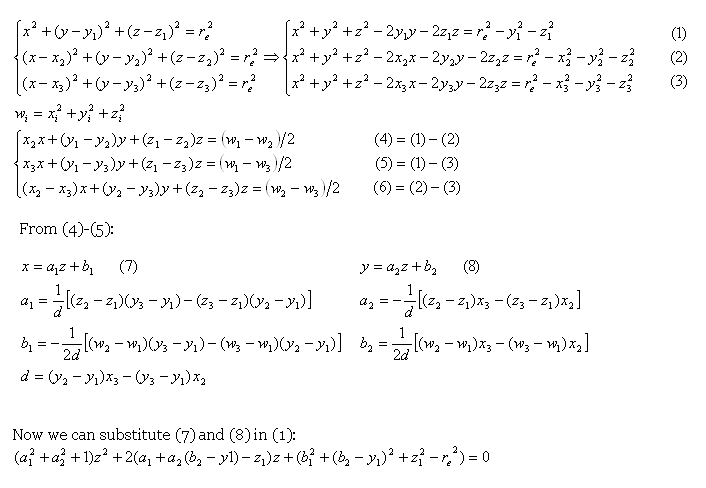
\includegraphics[width=0.4\linewidth]{deltamath.png}
     \quad
    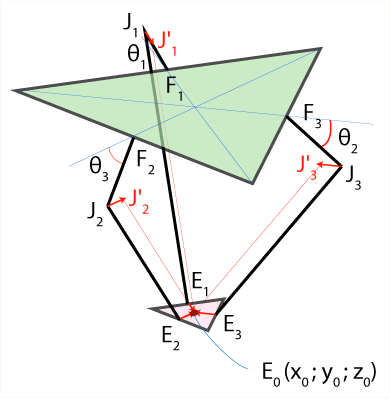
\includegraphics[width=0.4\linewidth]{delta.png}
  \end{figure}
 REMEMBER! DO NOT PANIC!
 \end{frame}
%----------------------------------------------------------------------------------------
\begin{frame}
  \frametitle{But let's see how that really works!}
  \begin{figure}
     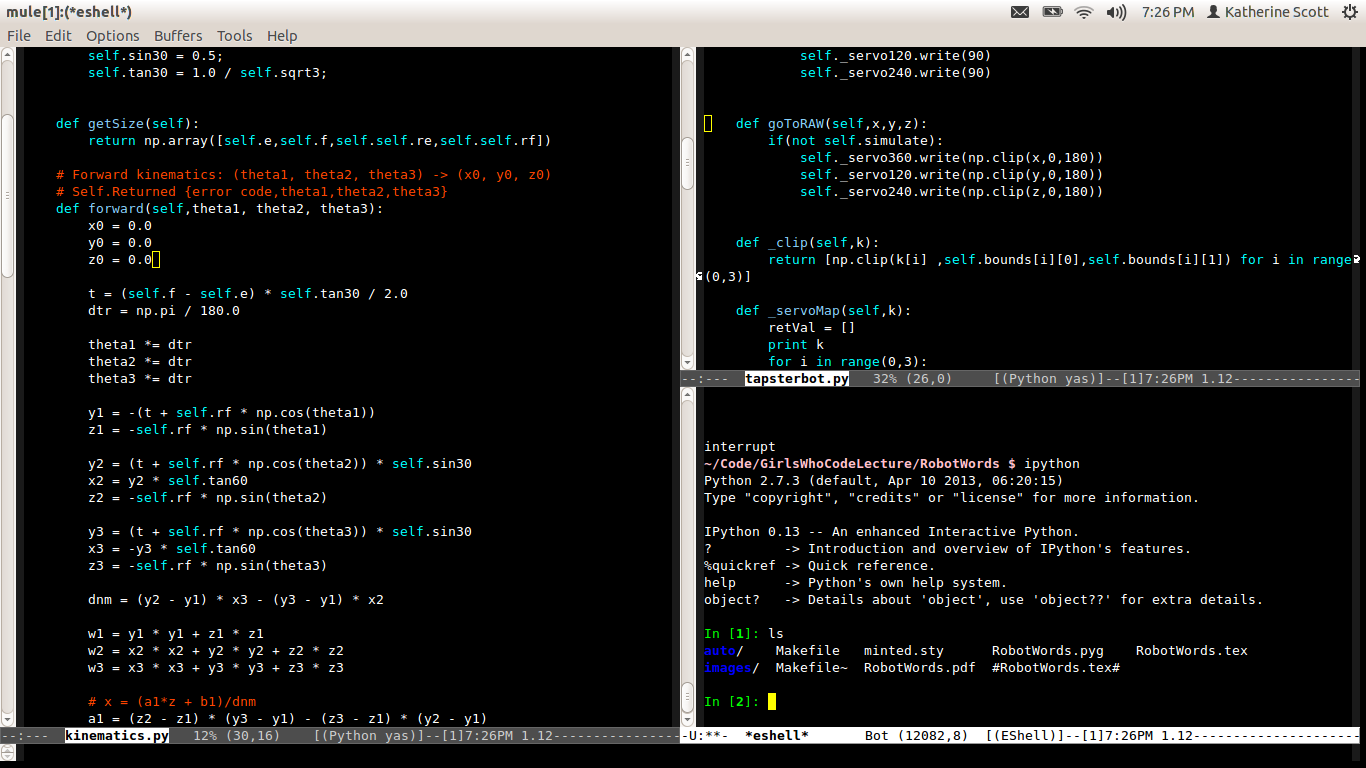
\includegraphics[width=0.8\linewidth]{emacs.png}
   \end{figure}
 \end{frame}

%----------------------------------------------------------------------------------------
\begin{frame}
  \frametitle{Controllers - More Fancy Words}
  \begin{figure}
     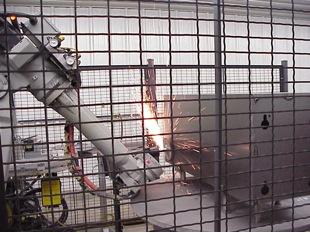
\includegraphics[width=0.4\linewidth]{caged.jpg}
     \quad
     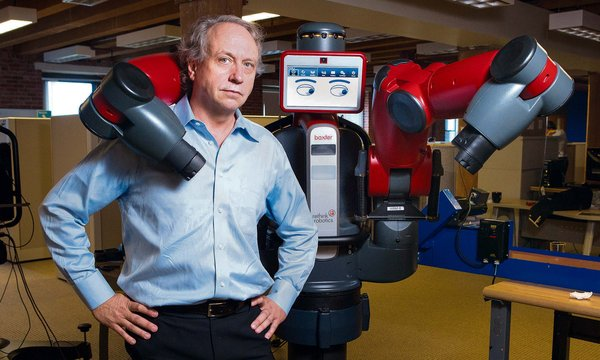
\includegraphics[width=0.4\linewidth]{rethink.jpg}
  \end{figure}
   \begin{itemize}
   \item \textbf{Closed-Loop Control} - We move the robot a bit, we check encoders, we move again. 
   \item \textbf{Open-Loop Control} - We just move the actuators. If they slip or we hit something too bad. 
   \item \textbf{PID Controller}  - Proportional Integral Derivative. An algorithm that uses calculus to do closed loop control. 
    \item \textbf{Kalman Filter} a way of estimating ``state'' given noisy measurements. 
   \end{itemize}     
 \end{frame}

%----------------------------------------------------------------------------------------
\begin{frame}
  \frametitle{Map Building and Path Planning}
  \begin{figure}
     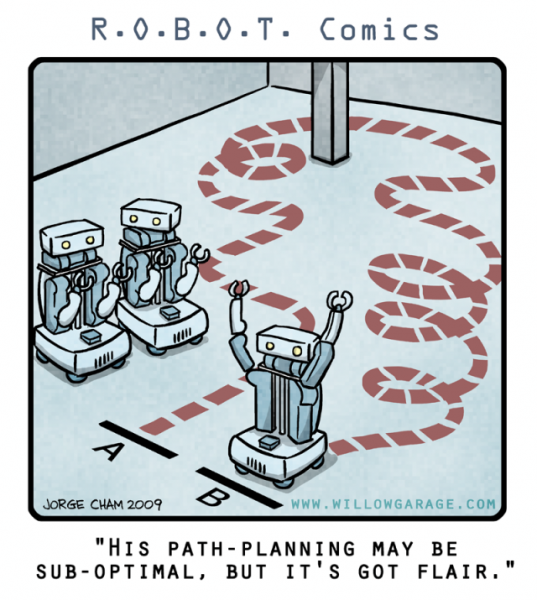
\includegraphics[width=0.4\linewidth]{suboptimal.png}
  \end{figure}
   \begin{itemize}
  \item \textbf{Mapping} is what allows a robot to plan a path. Map data comes from sensors or knowledge. 
   \item \textbf{Path Planning} - is the general name for the algorithms that help robots go from one point to another.

   \end{itemize}     
 \end{frame}
%----------------------------------------------------------------------------------------
\begin{frame}
  \frametitle{Mapping / Path Planning}
  \begin{figure}
     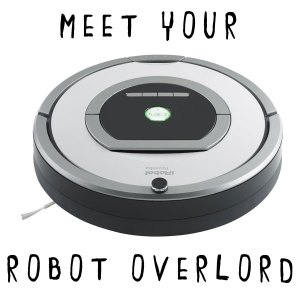
\includegraphics[width=0.2\linewidth]{overlord.jpg}
  \end{figure}
  \center{\href{http://www.youtube.com/watch?v=GPOe6uDOS_Q}{Roomba Path Planning}}
   \begin{itemize}
   \item The best way to get from A to B is not always a line. Stuff gets in your way.
   \item Path planning might be done to avoid \href{http://vimeo.com/20095999}{``singularies''} where our math does weird stuff.   
   \item \textbf{Dead Reckoning} is a simple path planning algorithm. Basically keep a list of heading and distance traveled. 
   \item What happens when we move one tapsterbot motor at a time versus all three at once? 
   \end{itemize}     
 \end{frame}

%----------------------------------------------------------------------------------------
\begin{frame}
  \frametitle{High Level Behavior}
  \begin{figure}
     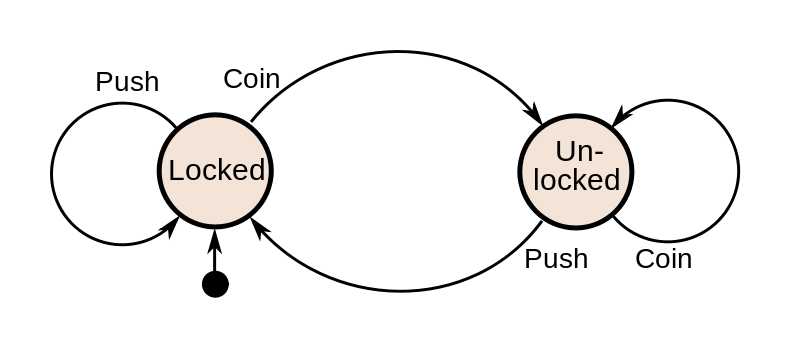
\includegraphics[width=0.4\linewidth]{statemachine.png}
  \end{figure}
  \center{\textit{A turnstile state machine,two states, two inputs.}}
   \begin{itemize}
     \item For beginners \textbf{finite state machines} are a good way to build up complex behaviors. 
     \item State Machines have \textbf{states} where the robot performs one set of behaviors. 
    \item State Machines also have \textbf{inputs} that cause \textbf{transitions} between states. 
    \item State Machines are a great way to break up and think about problems.
   \end{itemize}     
 \end{frame}

%----------------------------------------------------------------------------------------
\begin{frame}
  \frametitle{Hey, Let's Write Some Python Code for Tapsterbot}
  Let's create three states
  \begin{itemize}
  \item \textbf{WAIT} - Do nothing. 
  \item \textbf{DANCE} - Swing around.
  \item \textbf{PULL-UP} - Do some pull ups.
  \end{itemize}
  And tie those states to some inputs from a leap motion.
  \begin{itemize}
  \item Hand is open, let's do pull up.
  \item Hand is closed, let's dance. 
  \item Hand is not there, wait
  \end{itemize}
  
 \end{frame}


%------------------------------------------------

\begin{frame}
\begin{figure}
  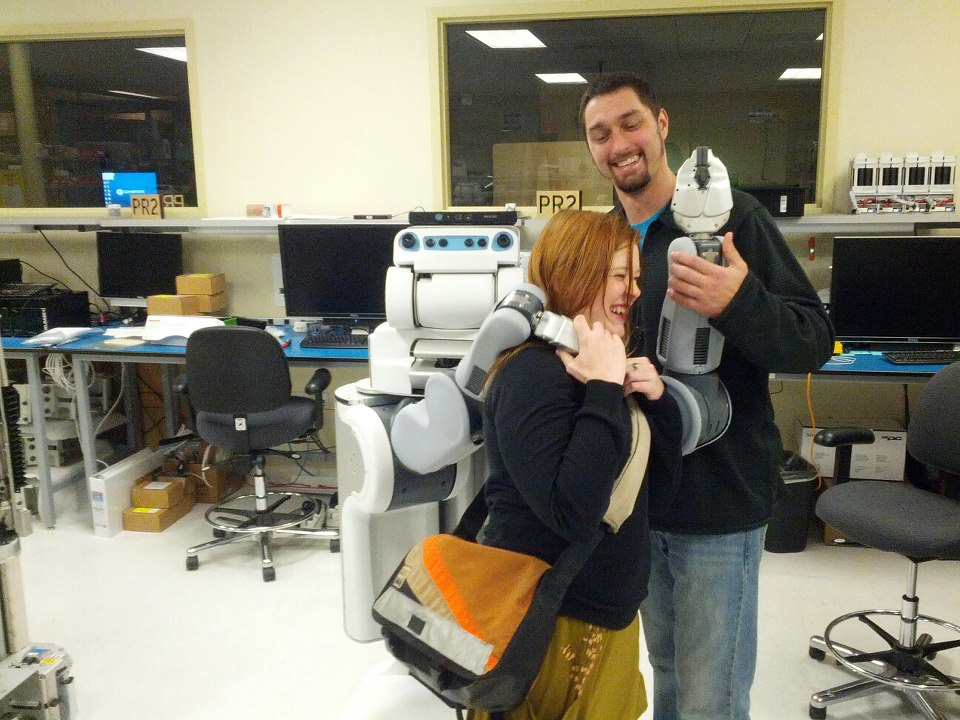
\includegraphics[width=0.4\linewidth]{katpr2.jpg}
\end{figure}
\Huge{\centerline{go hug a robot}}
\end{frame}

%----------------------------------------------------------------------------------------

\end{document} 
